% !Mode:: "TeX:UTF-8"
% !Mode:: "TeX:UTF-8"
\newcommand{\thepage}{} % to silence a hyperref warning about pdfpagelabels
\RequirePackage[]{silence}
\WarningsOff[hyperref]
\PassOptionsToPackage{log-declarations=false}{xparse}
%\RequirePackage[l2tabu, orthodox]{nag}
\RequirePackage{luatex85} % to make \pdf...= commands work with LuaTeX
\documentclass[aspectratio=169,t]{beamer}
\usepackage{ifthen}
\usepackage[T1]{fontenc}
\usepackage{iftex}
\ifLuaTeX
 \usepackage{fontspec}
 \setmainfont[Ligatures=TeX]{Source Sans Pro}
\else
 \usepackage[utf8]{inputenc}
\fi
\usepackage{german}
\usepackage{newunicodechar}
\newunicodechar{€}{\texteuro}
\newunicodechar{ß}{\ss}
\renewcommand{\SS}{\iffontchar\font"1E9E \symbol{"1E9E}\else SS\fi}
\usepackage{ellipsis}
\usepackage{microtype}
\usepackage{listings}
\usepackage{sourcecodepro}
\lstset{language=Python, basicstyle=\ttfamily}
\usepackage{amsfonts}
\usepackage{amssymb}
\usepackage{amsthm}
\usepackage{fancyhdr}
\usepackage{graphicx}

\newtheorem{proposition}[theorem]{Proposition}

\DeclareMathOperator*{\argmax}{argmax}
\DeclareMathOperator{\supp}{supp}
\newcommand{\E}{\ensuremath{\mathbb{E}}}
\newcommand{\V}{\ensuremath{\mathbb{V}}}

\setbeamercolor{emph}{fg=purple}
\renewcommand<>{\emph}[1]{%
  {\usebeamercolor[fg]{emph}\only#2{\itshape}#1}%
}



\hypersetup{draft=false,colorlinks=false,pdfpagemode=UseOutlines,plainpages=false,
            breaklinks=true,bookmarksnumbered=true,pdfborder=0 0 0,
            pdftitle={Data Science SoSe 2026 HHU},
            pdfauthor={Konrad Voelkel},
            pdfsubject={data science}}

%\documentclass[aspectratio=169,t]{beamer}
\usetheme{hhubeamer} % put the hhu-beamer-theme in /usr/share/texmf/tex/latex/beamer/themes/

% -------------------- Code listings config --------------------
% Define custom colors for syntax highlighting
\definecolor{codegreen}{rgb}{0,0.6,0}
\definecolor{codegray}{rgb}{0.5,0.5,0.5}
\definecolor{codepurple}{rgb}{0.58,0,0.82}
\definecolor{backcolour}{rgb}{0.96,0.96,0.94} % Very light gray/beige
% Configure the listings package
\lstset{
    language=Python,
    backgroundcolor=\color{backcolour},   
    commentstyle=\color{codegreen}\itshape,
    keywordstyle=\color{blue}\bfseries,
    numberstyle=\tiny\color{codegray},
    stringstyle=\color{codepurple},
    basicstyle=\ttfamily\footnotesize, % Use a monospaced font
    breakatwhitespace=false,         
    breaklines=true,      
             % Enable automatic line breaking
    captionpos=b,                      % Caption at the bottom
    keepspaces=true,                 
    numbers=left,                      % Line numbers on the left
    numbersep=10pt,                    % Distance of line numbers from the code
    showspaces=false,                
    showstringspaces=false,            % Don't show weird underscores in strings
    showtabs=false,                  
    tabsize=4,
    frame=single,                      % Add a subtle border around the code
    rulecolor=\color{black!20},        % Border color
  }

\event[]{}
\author[Sommersemester 2026]{Dr. Konrad Völkel, Sommersemester 2026}

%\title{Data Science, VL 1}
%\date{16.04.2026}


%%% Local Variables:
%%% mode: latex
%%% TeX-master: t
%%% End:


\title{Data Science, VL 5} % war in 2025 noch VL 4; Einschub zu Python kam dazwischen...
\date{30.04.2025}

\begin{document}

\begin{frame}
  \titlepage
\end{frame}


\section{Recap}

\begin{frame}
  \frametitle{Was bisher geschah: Statistik}
  \begin{itemize}[<+->]
  \item Für einen Vektor $v$ reeller Zahlen (eine Spalte in einer Tabelle Daten) lassen sich $median$ und $mean$ definieren wie üblich. Dabei minimiert ein Median den mittleren absoluten Fehler $mae$; das arithmetische Mittel ($mean$) minimiert den mittleren quadratischen Fehler $mse$ zu den Daten.
  \item Die Daten $v$ lassen sich \alert{zentrieren}: $\tilde{v} := v - mean(v)$. \\
    Dabei muss $- mean(v)$ komponentenweise verstanden werden, also $\tilde{v}_i := v_i - mean(v)$.
  \item Die Wurzel aus dem mittleren quadratischen Fehler des Mittelwerts heißt \alert{Sample-Standardabweichung} $\sigma(v) := rmse(v,mean(v)) = \frac{1}{\sqrt{n}} \Vert \tilde{v} \Vert$.
    \item Die \alert{Varianz} von $v$ ist $\sigma(v)^2 = \frac{1}{n} \tilde{v} \cdot \tilde{v} = \frac{1}{n} \tilde{v}^\top \tilde{v}$.
  \end{itemize}
\end{frame}

\begin{frame}
  \frametitle{Was bisher geschah: Stochastik}
  \begin{itemize}[<+->]
    \item Reelle \alert{Zufallsvariablen} sind (messbare) Abbildungen $X \colon \Omega \to \mathbb{R}$, die induzierte Verteilung $P_X$ heißt auch \alert{Verteilung von $X$} und lässt sich für endliche $\Omega$ mit einer \alert{pmf} beschreiben, $p_X(x) = P(X = x) = \sum_{\omega \in \Omega : X(\omega)=x} P_\Omega(\{\omega\})$.
    \item $\mathbb{E}(X) := \sum_{x \in \mathbb{R}} x p(x)$ heißt \alert{Erwartungswert} von $X$.
    \item $\mathbb{V}(X) := \mathbb{E}\left({\left(X-\mathbb{E}X\right)}^2\right) = \mathbb{E}(X^2) - {\left(\mathbb{E}X\right)}^2$ heißt \alert{Varianz} von $X$
  und\\
  $\sigma(X) := \sqrt{\mathbb{V}X}$ die \alert{Standardabweichung} von $X$.
  \end{itemize}
\end{frame}

   \begin{frame}
    \frametitle{Ausblick: Höhere Momente}
\begin{itemize}[<+->]
\item Für allgemeines $n$ ist $\mu_n(X) := \mathbb{E}\left( X^n \right)$ das \alert{$n$-te Moment},
 \item $\tilde{X} := X - \mathbb{E}(X)$ die \alert{zentrierte Zufallsvariable},
 \item  $\tilde{\mu}_n(X) := \mu_n(\tilde{X})$ das \alert{$n$-te zentrale Moment}.
   \item Es ist $\mu_1(X)=\mathbb{E}X$, $\tilde{\mu}_1(X) = 0$, $\tilde{\mu}_2(X) = \mathbb{V}X$.
\end{itemize}
\end{frame}


\subsection{Vektorisierung}

\begin{frame}
  \frametitle{Numpy}
  Wir werden im Folgenden das Paket Numpy verwenden, denn
  \begin{itemize}[<+->]
  \item Numpy bietet ein Interface zu schnellen Bibliotheken für lineare Algebra und Statistik, die in C, Fortran oder Assembler geschrieben sind.
  \item Numpy ermöglicht \alert{SIMD}-Verarbeitung: \alert{single instruction, multiple data}.\\
    \uncover<3->{
      Anstelle von expliziten for-Schleifen über Listen wird eine Operation auf einen ganzen Vektor angewendet.
      Wenn die Operation keine Verzweigungen (Branching, also if-Abfragen) enthält, kann ein moderner Prozessor das schneller.
    }
    \item PyTorch (für Deep Learning) arbeitet sehr ähnlich mit Vektoren (tensor vs. ndarray).
    \end{itemize}
    \uncover<4->{Wir müssen unseren Code also verzweigungsfrei gestalten, \alert{vektorisieren}.}
\end{frame}


\begin{frame}[separator]
  \frametitle{Pause?}
\end{frame}


\section{Stochastik programmieren}

\begin{frame}[separator]
  \frametitle{Programmierung}
\end{frame}

\begin{frame}
  \frametitle{Im Notebook: Stochastik programmieren}
\end{frame}


\section{Unabhängigkeit}

\begin{frame}
  \frametitle{Unabhängigkeit}
  \begin{definition}
    Sei $\Omega$ ein Wahrscheinlichkeitsraum.\\
    Ereignisse $A,B \subseteq \Omega$ heißen \alert{voneinander unabhängig}, wenn
$$
P(A\cap B) = P(A) \cdot P(B).
$$
\uncover<2->{
  Allgemeiner heißt eine Familie $(A_i)_{i\in I}$, $A_i \subseteq \Omega$ von Ereignissen \alert{unabhängig},\\
  wenn für jede endliche Teilindexmenge $J \subseteq I$ gilt:
$$
P\left( \bigcap_{j \in J} A_j \right) = \prod_{j\in J} P(A_j).
$$
}
\end{definition}
\end{frame}

\begin{frame}
  \frametitle{Beispiel zur Unabhängigkeit}
\uncover<+->{  
  Zwei faire sechsseitige Würfel werden unabhängig voneinander geworfen.

  \begin{itemize}
    \item Ereignis $A$: Der erste Würfel zeigt eine gerade Zahl.
    \item Ereignis $B$: Der zweite Würfel zeigt eine $6$.
    \end{itemize}
    }
    
\uncover<+->{
  \vspace{1em}
  \begin{itemize}
    \item $P(A) = \frac{3}{6} = \frac{1}{2}$ \quad (gerade Zahlen: 2, 4, 6)
    \item $P(B) = \frac{1}{6}$
    \item $P(A \cap B) = P(A) \cdot P(B) = \frac{1}{2} \cdot \frac{1}{6} = \frac{1}{12}$
    \end{itemize}
    }

    \uncover<+->{
  \vspace{1em}
  Da $A$ und $B$ sich auf unterschiedliche Würfel beziehen, sind sie \alert{unabhängig}.
  }
\end{frame}

\begin{frame}
  \frametitle{Beispiel zur Abhängigkeit}


\vspace{-0.3cm}
  
    \uncover<+->{
  Eine Tüte enthält je ein rotes, grünes und blaues Bonbon.\\
  Zwei Bonbons werden nacheinander \alert{ohne Zurücklegen} gezogen.
}

\vspace{0.3cm}

    \uncover<+->{
  \begin{itemize}
    \item Ereignis $A$: Das erste gezogene Bonbon ist rot.
    \item Ereignis $B$: Das zweite gezogene Bonbon ist grün.
  \end{itemize}
}


    \uncover<+->{
  Insgesamt gibt es $3 \cdot 2 = 6$ mögliche geordnete Ziehungen.
}

  \begin{itemize}[<+->]
    \item Zustände für $A$: (rot, grün), (rot, blau) $\Rightarrow P(A) = \frac{2}{6} = \frac{1}{3}$
    \item Zustände für $B$: (rot, grün), (blau, grün) $\Rightarrow P(B) = \frac{2}{6} = \frac{1}{3}$
    \item Zustände für $A \cap B$: (rot, grün) $\Rightarrow P(A \cap B) = \frac{1}{6}$
  \end{itemize}

      \uncover<+->{
  \[
    P(A) \cdot P(B) = \frac{1}{3} \cdot \frac{1}{3} = \frac{1}{9} \ne \frac{1}{6} = P(A \cap B)\]

\[    \Rightarrow \quad
    A \text{ und } B \text{ sind also \alert{nicht unabhängig}, sie sind \alert{abhängig}}.   \]
  }
\end{frame}

\begin{frame}
  \frametitle{Unabhängige Zufallsvariablen}
  \begin{definition}
    Sei $\Omega$ ein Wahrscheinlichkeitsraum, dann heißen zwei Zufallsvariablen $X \colon \Omega_X' \to \Omega_X,\ Y \colon \Omega_Y' \to \Omega_Y$ \alert{unabhängig}, wenn
    für alle $A \subseteq \Omega_X$ und $B \subseteq \Omega_Y$ gilt:
    \[P(X \in A,\ Y \in B) = P(X \in A)\cdot P(Y \in B).\]
\uncover<2->{
  Dabei bedeutet $P(X \in A,\ Y \in B) = P((X,Y) \in A \times B)$\\
  für die \alert{gemeinsame Verteilung} von $(X,Y) \colon \Omega_X' \times \Omega_Y' \to \Omega_X \times \Omega_Y$.
}

\uncover<3->{
  Wenn $X$ eine pmf $p$ und $Y$ eine pmf $q$ hat,\\
  dann sind $X$ und $Y$ unabhängig genau dann, wenn
  \[P(X = x, Y = y) = p(x)q(y).\]
}
%  Achtung: i.A. ist $p \cdot q$ keine pmf für die gemeinsame Verteilung $(X,Y)$.
\end{definition}
\end{frame}

\begin{frame}
  \frametitle{Korrelation}
  Achtung: \uncover<+->{Abhängigkeit $\neq$ Korrelation!}

  \uncover<2->{Korrelation $\Rightarrow$ Abhängigkeit}

  \uncover<3->{Korrelation misst man mit dem Korrelationskoeffizienten, der Kovarianz.
    
    Abhängigkeit lässt sich mit der relativen Entropie messen.

  Das besprechen wir beides noch, auf dem Weg zur multivariaten Statistik.}
\end{frame}


\begin{frame}[separator]
  \frametitle{Pause?}
  
  \vspace{-2.2cm}
  \hspace{-0.8cm}
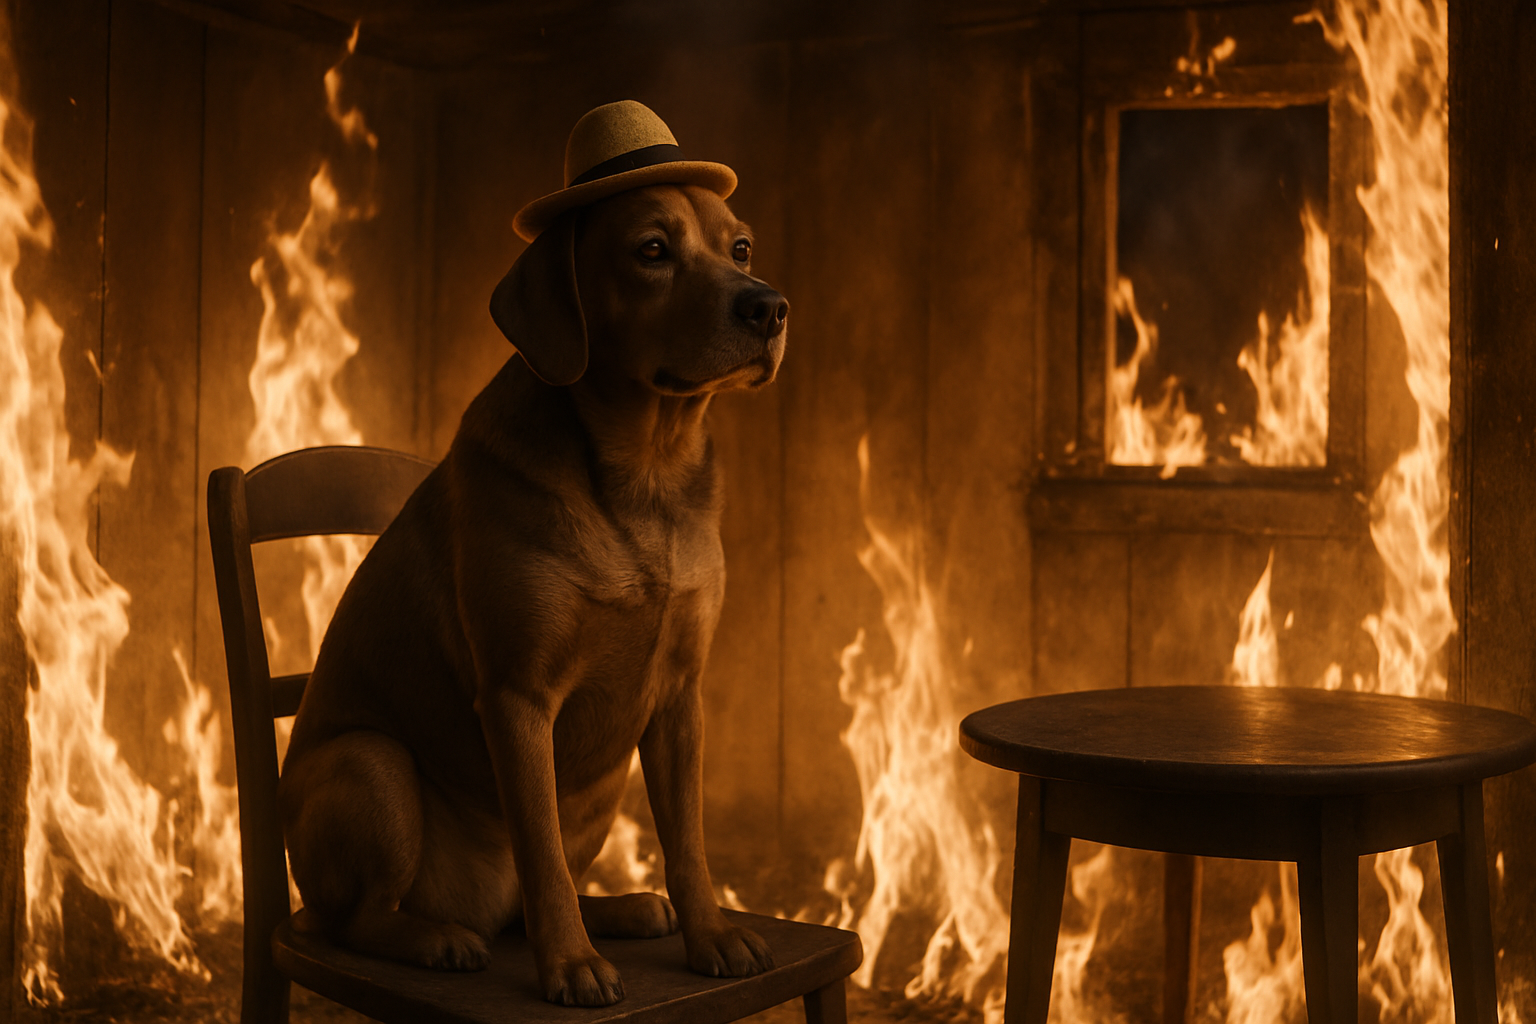
\includegraphics[scale=0.22]{figures/this-is-fine.png}
\end{frame}

\section{Sätze: Markov, Tschebyscheff, Große Zahlen}

\begin{frame}
  \frametitle{Motivation: Das Gesetz der großen Zahlen}

\begin{itemize}[<+->]
\item Setup:  Wir wiederholen ein Zufallsexperiment (Zufallsvariable $X \colon \Omega \to \mathbb{R}$)

\vspace{0.6cm}
  
\item Modell: Eine Folge von Zufallsvariablen $X_1,\ X_2,\ \dots$ mit $X_i \sim X$
  
\item $X_i \sim X$ := ``Jedes $X_i$ ist \alert{verteilt wie $X$}''.
  
\item Außerdem: $X_i$ beeinflusst $X_{i+1}$ nicht usw. ``\alert{Unabhängigkeit}''

\vspace{0.6cm}
  
\item ``Satz'':  Dann konvergiert der Mittelwert von $X_1,\dots,X_n$ gegen $\mathbb{E}X$.
  
\item Interpretation: Je größer die Stichprobe, desto besser schätzt \texttt{mean} den $\mathbb{E}X$.
\end{itemize}
\vspace{0.6cm}

Wir üben die bisher gelernten Konzepte, indem wir eine Beweisskizze anschauen.
\end{frame}

       \begin{frame}
    \frametitle{Markov}
    \begin{lemma}[Markov-Ungleichung]
      Für $X \colon \Omega \to \mathbb{R}$ mit $X \geq 0$ und $a > 0$ ist
 \[P(X \geq a) \ \leq\ \frac{\mathbb{E} X}{a}\]
\end{lemma}
\begin{proof}[Beweis]<2->
  \[\mathbb{E}X = \sum_{x=-\infty}^{\infty} x\ p(x) \uncover<3->{\overset{(X \geq 0)}{=}  \sum_{x=0}^{\infty} x\ p(x)} \uncover<4->{ \geq \sum_{x=a}^\infty x\ p(x)} \uncover<5->{\geq \sum_{x=a}^\infty a\ p(x)} \uncover<6->{= aP(X\geq a).}\]
  \uncover<6->{\qedhere}
\end{proof}
\end{frame} 

       \begin{frame}
    \frametitle{Tschebyscheff}
    \begin{lemma}[Tschebyscheff-Ungleichung]
 Für $\lambda > 0$ ist
 $P\left(\left|X - \mathbb{E}(X)\right| \geq \lambda \sigma(X)\right) \leq \frac{1}{\lambda^2}$.
\end{lemma}
\begin{proof}[Beweis]<2-> Wir wenden Markov-Ungleichung auf $Y := {\left(X - \mathbb{E}X\right)}^2 \geq 0$ und $a := \lambda^2 \sigma(X)^2$ an:
  \[P\left({\left(X - \mathbb{E}X\right)}^2 \geq \lambda^2 \sigma(X)^2\right) \ \leq\ \frac{\mathbb{E} Y}{\lambda^2 \sigma(X)^2}\]
  \uncover<3->{
    Die Ungleichung $P\left( (\cdot )^2 \leq (\cdot )^2 \right)$ auf der linken Seite ist äquivalent zu $P\left( |\cdot | \leq |\cdot | \right)$.}
  
  \uncover<4->{Wir beobachten auf der rechten Seite noch $\mathbb{E}Y = \sigma(X)^2$. \qedhere}
  \end{proof}
\end{frame}

   \begin{frame}
    \frametitle{Gesetz der großen Zahlen}
    Für eine Zufallsvariable $X \colon \Omega \to \mathbb{R}$ mit existierendem Erwartungswert,\\
    genügt eine Folge unabhängiger Zufallsvariablen $X_i$ mit $X \sim X_i$\\
    (\alert{unabhängig identisch verteilt, iid}) einem \alert{starken Gesetz der großen Zahlen}:

    Die Mittelwert-Abweichungs-Zufallsvariablen $\overline{X}_n - \mathbb{E}X  = \frac{1}{n} \sum_{i=1}^n (X_i - \mathbb{E}X_i)$ ``konvergieren $P$-fast sicher gegen $0$'', d.h.
    \[P\left(\lim_{n\to \infty} \overline{X}_n = \mathbb{E}X\right) = 1.\]
    \uncover<2->{
      Daraus folgt auch die ``stochastische Konvergenz'': für jedes $\epsilon > 0$ ist
      \[\lim_{n\to\infty} P\left( |\overline{X}_n-\mathbb{E}X| \geq \epsilon \right) = 0\]
      }
    \end{frame}

       \begin{frame}
    \frametitle{Beweisskizze Große Zahlen}
    \begin{proof}[Beweisskizze schwaches Gesetz der großen Zahlen 1/2]
      (Mit $\mu := \mathbb{E}X = \mathbb{E}X_i$ unter der Annahme endlicher Varianz $\mathbb{V}X_i = \mathbb{V}X =: \sigma^2$)
      \[\uncover<+->{\mathbb{V}\left(\overline{X}_n\right) = \mathbb{V}\left( \frac{1}{n} \sum_{i=1}^n \left(X_i - \mathbb{E}X_i\right) \right)}  \uncover<+->{= \frac{1}{n^2} \mathbb{V}\left( \left(\sum_{i=1}^n X_i\right) - n\mathbb{E}X \right)} \uncover<+->{= \frac{1}{n^2} \mathbb{V}\left( \sum_{i=1}^n X_i \right)}\]
      \uncover<+->{Weil die $X_i$ unabhängig sind, lässt sich auch die Summe herausziehen:}
        \[ \phantom{\frac{1}{n^2} \mathbb{V}\left( \sum_{i=1}^n X_i \right)} \uncover<+->{= \frac{1}{n^2} \sum_{i=1}^n \mathbb{V}\left( X_i \right)} \uncover<+->{= \frac{n}{n^2} \mathbb{V}X} \uncover<+->{= \frac{\sigma^2}{n}.}\]
        \phantom\qedhere % (da ist der Beweis noch nicht zuende)
    \vspace{4cm}  \phantom{text}
  \end{proof}
\end{frame}

\begin{frame}
    \frametitle{Beweisskizze Große Zahlen}
    \begin{proof}[Beweisskizze schwaches Gesetz der großen Zahlen 2/2]
      (Mit $\mu := \mathbb{E}X = \mathbb{E}X_i$ unter der Annahme endlicher Varianz $\mathbb{V}X_i = \mathbb{V}X =: \sigma^2$)
      \[ \uncover<+->{\mathbb{V}\left(\overline{X}_n\right) = \frac{\sigma^2}{n},} \qquad  \uncover<+->{\mathbb{E} \overline{X}_n = \mathbb{E} \left( \frac{1}{n} \sum_{i=1}^n X_i \right)}  \uncover<+->{= \frac{1}{n} \sum_{i=1}^n \mathbb{E}X_i} \uncover<+->{ = \frac{n}{n}\mu = \mu.}\]
      \uncover<+->{Wir wenden die Tschebyscheff-Ungleichung auf $\overline{X}_n$ an:
        \[P\left(\left|\overline{X}_n - \mu \right| \geq \varepsilon\right) \leq \frac{\sigma^2}{n\varepsilon^2} \xrightarrow{n \to \infty} 0.\]}
      \uncover<+->{
      Das ist genau die stochastische Konvergenz. \qedhere}
    \end{proof}
  \end{frame}





\begin{frame}[separator]
  \frametitle{Vielen Dank für Ihre Aufmerksamkeit!}
\end{frame}

\end{document}

%%% Local Variables:
%%% mode: latex
%%% TeX-master: t
%%% End:
